\begin{table}[ht!]
\centering
\scriptsize
\setlength{\tabcolsep}{3pt}
\renewcommand{\arraystretch}{1.1}
\caption{Scoring criteria for the part of GM-100 benchmark tasks.}
\label{tab:bm_scoring}
\begin{tabular}{p{0.12\columnwidth} p{0.22\columnwidth} p{0.56\columnwidth}}
\toprule
\textbf{Task ID} & \textbf{Task} & \textbf{Scoring Criteria} \\
\midrule

BM-19 & Block Sorting &
\makecell[l]{
1. Pick up the largest block on the table (16). \\
2. Place the largest block on the far left (12). \\
3. Pick up the second-largest block on the table (12). \\
4. Place the second-largest block to the right of the largest block (12). \\
5. Pick up the third-largest block on the table (12). \\
6. Place the third-largest block to the right of the second-largest block (12). \\
7. Pick up the smallest block on the table (12). \\
8. Place the smallest block on the far right (12).
} \\
\midrule

BM-20 & Retrieve Keychain &
\makecell[l]{
1. Pull open the drawer (25). \\
2. Grasp the keychain (25). \\
3. Move the keychain to the front of the drawer (25). \\
4. Put down the keychain (25).
} \\
\midrule

BM-25 & Scoop Rice &
\makecell[l]{
1. Pick up the spoon with the right hand (20). \\
2. Scoop rice from the bowl with the spoon (30). \\
3. Pour the rice into the cup (30). \\
4. Place the spoon back onto the plate (20).
} \\
\midrule

BM-39 & Replace Paper Roll &
\makecell[l]{
1. Remove the empty paper-roll core (22). \\
2. Place the core on the tray (22). \\
3. Pick up the new paper roll (22). \\
4. Install the new paper roll onto the holder (34).
} \\
\midrule

BM-45 & Sort Snacks &
\makecell[l]{
1. Pick up the first type of snack (18). \\
2. Place it into the corresponding container (16). \\
3. Pick up the second type of snack (17). \\
4. Place it into the corresponding container (16). \\
5. Pick up the third type of snack (17). \\
6. Place it into the corresponding container (16).
} \\
\midrule

BM-47 & Pack Eggs &
\makecell[l]{
1. Pick up the first egg (16). \\
2. Place the egg into a tray slot (12). \\
3. Pick up the second egg (12). \\
4. Place the egg into a tray slot (12). \\
5. Pick up the third egg (12). \\
6. Place the egg into a tray slot (12). \\
7. Pick up the fourth egg (12). \\
8. Place the egg into a tray slot (12).
} \\
\midrule

BM-69 & Pick Out Toy Bones &
\makecell[l]{
1. Pick up the first toy bone (25). \\
2. Move the bone out of the plate (25). \\
3. Pick up the second toy bone (25). \\
4. Move the bone out of the plate (25).
} \\
\midrule

BM-75 & Push Ball into Box &
\makecell[l]{
1. Push the ball toward the box (30). \\
2. Push the ball into the box (70).
} \\
\midrule

BM-82 & Squeeze Ketchup &
\makecell[l]{
1. Pick up the ketchup bottle with the left hand and hold it above the plate (25). \\
2. Tilt the bottle so that the nozzle points toward the plate (25). \\
3. Squeeze the bottle with both hands to dispense ketchup (25). \\
4. Put down the ketchup bottle (25).
} \\
\midrule

BM-97 & Take Bowl out of Microwave &
\makecell[l]{
1. Open the microwave door (25). \\
2. Grasp the bowl inside the microwave (25). \\
3. Move the bowl onto the table and place it down (25). \\
4. Close the microwave door (25).
} \\
\midrule

BM-105 & Tool Packing &
\makecell[l]{
1. Pick up the tape and place it into the toolbox (20). \\
2. Pick up the measuring tape and place it into the toolbox (20). \\
3. Pick up the screwdriver and place it into the toolbox (20). \\
4. Pick up the cutter and place it into the toolbox (20). \\
5. Close the toolbox (20).
} \\
\midrule

BM-107 & Barcode Scan &
\makecell[l]{
1. Lift the medicine box and hold it up with the left hand (20). \\
2. Pick up the barcode scanner with the right hand (20). \\
3. Scan the barcode on the medicine box with the scanner (20). \\
4. Put down the barcode scanner (20). \\
5. Put the medicine box back down (20).
} \\

\bottomrule
\end{tabular}
\end{table}

\section{Experiments}\label{sec:exp}

\subsection{Experimental Settings}

\noindent\textbf{Scoring criteria.} 
\Cref{tab:bm_scoring} summarizes the scoring criteria for a subset of GM-100 benchmark tasks. Each task is decomposed into a sequence of fine-grained manipulation steps, and a partial score is assigned to each step according to task completion. These criteria cover diverse bimanual capabilities, including sorting, retrieval, scooping, replacement, packing, pushing, squeezing, and coordinated object handling. Such stepwise annotations enable a more fine-grained evaluation than binary success alone, capturing partial progress on long-horizon manipulation tasks.

\subsection{Bimanual Manipulation Experiment Results}

\begin{table*}[h]
\centering
\small
\setlength{\tabcolsep}{4.2pt}
\renewcommand{\arraystretch}{1.08}
\caption{
Performance on the bimanual GM-100 benchmark under the generalist setting.
We report progress score (Prog., \%) and success rate (Succ., \%) for each task.
The shaded row in each platform block reports the average over the nine tasks.
}
\label{tab:bimanual_combined}
\begin{tabular}{@{}lrrrrrrrr@{}}
\toprule
\multirow{2}{*}{Task} &
\multicolumn{2}{c}{GR00T N1.7} &
\multicolumn{2}{c}{$\pi_{0.5}$} &
\multicolumn{2}{c}{LingBot-VLA-1.0} &
\multicolumn{2}{c}{LingBot-VLA-2.0} \\
\cmidrule(lr){2-3}
\cmidrule(lr){4-5}
\cmidrule(lr){6-7}
\cmidrule(l){8-9}
& Prog. & Succ. & Prog. & Succ. & Prog. & Succ. & Prog. & Succ. \\
\midrule

\multicolumn{9}{@{}l}{\textbf{Agilex Cobot Magic}} \\
\rowcolor{gray!8}
\textbf{Overall average}
& 36.3 & 17.8 & 59.1 & 32.2 & 58.2 & 30.0 & \textbf{66.2} & \textbf{34.4} \\

Block sorting              
& 40.0 & 10.0 & 90.4 & 60.0 & 59.2 & 10.0 & 56.8 & 0.0 \\
Retrieve keychain          
& 12.5 & 10.0 & 20.0 & 20.0 & 67.5 & 60.0 & 100.0 & 100.0 \\
Replace paper roll         
& 52.8 & 0.0 & 62.8 & 10.0 & 59.6 & 20.0 & 55.2 & 20.0 \\
Sort snacks                
& 91.9 & 70.0 & 82.4 & 30.0 & 74.4 & 10.0 & 66.2 & 10.0 \\
Pack eggs                  
& 14.4 & 0.0 & 72.4 & 20.0 & 42.4 & 10.0 & 44.4 & 0.0 \\
Pick out toy bone          
& 70.0 & 60.0 & 100.0 & 100.0 & 77.5 & 70.0 & 95.0 & 90.0 \\
Push ball into box         
& 18.0 & 0.0 & 38.0 & 20.0 & 6.0 & 0.0 & 41.0 & 20.0 \\
Take bowl out of microwave 
& 15.0 & 10.0 & 0.0 & 0.0 & 77.5 & 70.0 & 77.5 & 70.0 \\
Tool packing               
& 12.0 & 0.0 & 66.0 & 30.0 & 60.0 & 20.0 & 60.0 & 0.0 \\

\addlinespace[0.35em]
\midrule

\multicolumn{9}{@{}l}{\textbf{Galaxea R1 Pro}} \\
\rowcolor{gray!8}
\textbf{Overall average}
& 16.4 & 5.6 & 27.4 & 8.9 & 32.7 & \textbf{15.6} & \textbf{34.6} & \textbf{15.6} \\

Block sorting              
& 8.4 & 0.0 & 12.4 & 0.0 & 28.0 & 0.0 & 33.2 & 0.0 \\
Retrieve keychain          
& 0.0 & 0.0 & 0.0 & 0.0 & 0.0 & 0.0 & 0.0 & 0.0 \\
Replace paper roll         
& 6.6 & 0.0 & 72.0 & 50.0 & 44.0 & 0.0 & 57.6 & 40.0 \\
Sort snacks                
& 31.3 & 0.0 & 28.1 & 0.0 & 10.6 & 0.0 & 26.1 & 0.0 \\
Pack eggs                  
& 1.6 & 0.0 & 6.7 & 0.0 & 19.2 & 0.0 & 4.4 & 0.0 \\
Pick out toy bone          
& 77.5 & 50.0 & 72.5 & 30.0 & 62.5 & 40.0 & 87.5 & 70.0 \\
Push ball into box         
& 9.0 & 0.0 & 21.0 & 0.0 & 3.0 & 0.0 & 18.0 & 0.0 \\
Take bowl out of microwave 
& 7.5 & 0.0 & 7.5 & 0.0 & 97.5 & 100.0 & 65.0 & 30.0 \\
Tool packing               
& 6.0 & 0.0 & 26.0 & 0.0 & 30.0 & 0.0 & 20.0 & 0.0 \\

\bottomrule
\end{tabular}
\end{table*}

\noindent\textbf{Experiment settings.}
We evaluate bimanual manipulation on nine tasks from the GM-100 benchmark under a generalist mixed-training setting. Unlike task-specific training, a single policy is jointly trained on all tasks for each embodiment, requiring the model to share manipulation primitives across diverse bimanual skills, including sorting, retrieval, packing, pushing, and articulated-object interaction. We report the progress score and success rate for each task.

\noindent\textbf{Results analysis.}
As shown in~\cref{tab:bimanual_combined}, LingBot-VLA-2.0 achieves the best overall performance under the generalist setting. On Agilex Cobot Magic, it reaches 66.2 / 34.4 in progress score / success rate, surpassing LingBot-VLA-1.0 by 8.0 / 4.4 points and $\pi_{0.5}$ by 7.1 / 2.2 points. On Galaxea R1 Pro, it achieves 34.6 / 15.6, outperforming $\pi_{0.5}$ by 7.2 / 6.7 points. These results demonstrate that LingBot-VLA-2.0 benefits from mixed-task training and acquires more generalizable bimanual manipulation behaviors.

The improvements are most pronounced on tasks that demand accurate object grounding and goal-directed action execution. For instance, on Agilex \textit{Retrieve keychain}, LingBot-VLA-2.0 improves over LingBot-VLA-1.0 from 67.5 / 60.0 to 100.0 / 100.0, and on Agilex \textit{Pick out toy bone}, from 77.5 / 70.0 to 95.0 / 90.0. A similar gain is observed on the Galaxea \textit{Pick out toy bone} task, where the performance increases from 62.5 / 40.0 to 87.5 / 70.0. These improvements align well with the design of LingBot-VLA-2.0, which adopts a stronger VLM backbone with enhanced grounding capability and conditions action prediction on future information, together enabling more object-centric and goal-consistent manipulation.

Nevertheless, the gains are not uniform across tasks. Several tasks still exhibit a substantial gap between progress score and success rate, indicating that the model often makes partial progress but fails at the final precise placement, release, or completion step. Moreover, the performance disparity between Agilex Cobot Magic and Galaxea R1 Pro suggests that embodiment-specific factors, such as kinematics, camera viewpoints, and action-space alignment, remain challenging. Overall, LingBot-VLA-2.0 delivers consistent improvements in generalist bimanual manipulation, particularly on tasks requiring strong visual grounding and future-aware action planning.

\subsection{Long-Horizon Mobile Manipulation Experiment Results}

\begin{figure}[t]
\centering
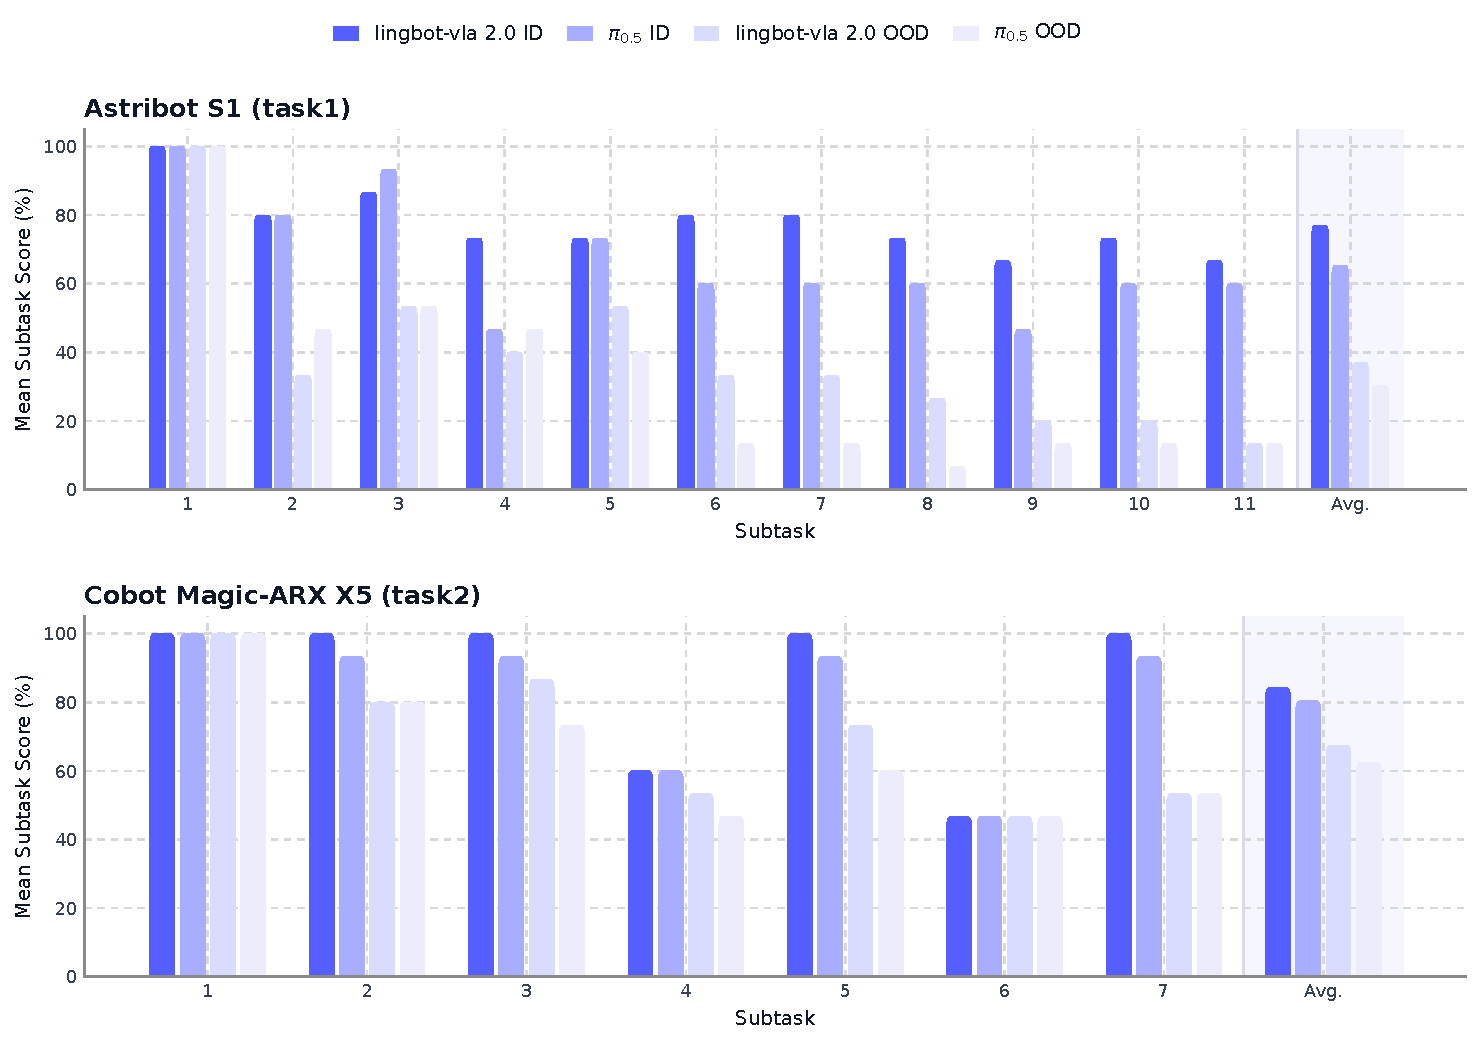
\includegraphics[width=\linewidth]{figures/bm_subtask_progress_domain_bar.pdf}
\caption{Per-subtask performance on the long-horizon mobile manipulation benchmark. Bars report the mean subtask completion score (\%) across 15 trials under both in-domain (ID) and out-of-distribution (OOD) settings.}
\label{fig:bm_subtask_progress_domain_bar}
\end{figure}

\begin{table}[h]
  \centering
  \caption{Long-horizon mobile manipulation benchmark results, reported as progress score / success rate (\%).}
  \label{tab:bm_results}
  \begin{tabular}{lllcc}
  \toprule
  Embodiment & Task & Setting & LingBot-VLA-2.0 & $\pi_{0.5}$ \\
  \midrule
  \multirow{2}{*}{Astribot S1}
  & \multirow{2}{*}{Sort objects into refrigerator}
  & In-domain & 77.1 / 60.0 & 65.3 / 46.7 \\
  & & Out-of-distribution & 37.0 / 13.3 & 30.3 / 6.7 \\
  \midrule
  \multirow{2}{*}{Cobot Magic-ARX X5}
  & \multirow{2}{*}{Stove cleaning}
  & In-domain & 84.3 / 66.7 & 79.9 / 60.0 \\
  & & Out-of-distribution & 67.5 / 40.0 & 62.5 / 33.3 \\
  \bottomrule
\end{tabular}
\end{table}

\noindent\textbf{Experiment settings.} We evaluate long-horizon mobile manipulation performance on two robotic embodiments, as illustrated in ~\cref{fig:bm_mobile_tasks}. Each embodiment is associated with one representative task: Astribot S1 is evaluated on the object sorting task, where objects are collected and placed into a refrigerator, while Cobot Magic-ARX X5 is evaluated on the stove cleaning task. The detailed sub-task decomposition and corresponding scoring criteria for each task are listed in ~\cref{tab:bm_scoring_mobile}.
For each task, we evaluate each model under two settings: in-domain (ID) and out-of-distribution (OOD). Each task-setting pair is evaluated with 15 independent trials. In the in-domain setting, both the robot initial position and the manipulated objects are drawn from the training distribution. In the out-of-distribution setting, the robot initial position is perturbed within ±10 cm along the forward, backward, left, and right directions around the nominal initial pose. In addition, for the refrigerator sorting task, the two fruits and the water bottle to be placed into the refrigerator are replaced with unseen object categories. This setting is designed to evaluate the model’s generalization ability under unseen object and position conditions.

\noindent\textbf{Results analysis.} As shown in~\cref{tab:bm_results}, LingBot-VLA-2.0 consistently outperforms $\pi_{0.5}$ across both robotic embodiments and both evaluation settings. In the in-domain setting, LingBot-VLA-2.0 achieves a progress score / success rate of 77.1 / 60.0 on the refrigerator sorting task and 84.3 / 66.7 on the stove cleaning task, improving over $\pi_{0.5}$ by 11.8 / 13.3 and 4.4 / 6.7 points, respectively. These results indicate that LingBot-VLA-2.0 can better execute long-horizon task sequences that require coordinated base movement, object manipulation, and interaction with articulated objects.
Under the OOD setting, both models exhibit performance degradation, reflecting the increased difficulty introduced by perturbed initial robot poses and unseen manipulated objects. Nevertheless, LingBot-VLA-2.0 maintains a clear advantage over $\pi_{0.5}$, achieving 37.0 / 13.3 on the refrigerator-sorting task and 67.5 / 40.0 on the stove-cleaning task. Compared with $\pi_{0.5}$, this corresponds to improvements of 6.7 / 6.6 and 5.0 / 6.7 points, respectively. The performance gap is especially meaningful in terms of success rate, suggesting that LingBot-VLA-2.0 is more robust in completing full task trajectories rather than only making partial progress.
The refrigerator sorting task shows a larger drop from the in-domain to the out-of-distribution setting than the stove cleaning task. This is expected because the out-of-distribution refrigerator setting simultaneously changes both the initial robot pose and the manipulated object categories, requiring stronger object-level generalization and more precise long-horizon recovery. In contrast, the stove cleaning task mainly evaluates robustness to initial pose perturbations while preserving the task objects and scene structure. Overall, the results demonstrate that LingBot-VLA-2.0 achieves stronger long-horizon mobile manipulation capability and better generalization than $\pi_{0.5}$ across both embodiments.




\begin{figure}[h!]
\centering

\begin{minipage}[t]{0.55\textwidth}
\vspace{0pt}
\centering
\scriptsize
\setlength{\tabcolsep}{3pt}
\renewcommand{\arraystretch}{1.1}
\captionof{table}{Scoring criteria for the long-horizon mobile manipulation experiment tasks.}
\label{tab:bm_scoring_mobile}
\begin{tabular}{p{0.18\linewidth} p{0.78\linewidth}}
\toprule
\textbf{Task} & \textbf{Scoring Criteria} \\
\midrule

Sort objects into refrigerator &
\makecell[l]{
1. Move from the initial position to the kitchen island (6). \\
2. Pick up the drink from the table and place it into the basket (9). \\
3. Pick up the first fruit from the table and place it into the basket (9). \\
4. Pick up the second fruit from the table and place it into the basket (11). \\
5. Pick up and lift the basket (8). \\
6. Move to the front of the refrigerator (10). \\
7. Open the refrigerator door wide enough to place items inside (12). \\
8. Pick up the first fruit and place it into the refrigerator (9). \\
9. Pick up the second fruit and place it into the refrigerator (11). \\
10. Pick up the drink and place it into the refrigerator (9). \\
11. Close the refrigerator door (6).
} \\
\midrule

Stove Cleaning &
\makecell[l]{
1. Move from the initial position to the front of the stove (8). \\
2. Pick up the black pot rack and place it on the left side of the table (16). \\
3. Pick up the sponge (12). \\
4. Wipe off the white foam on the stove using the sponge (18). \\
5. Transfer the sponge and place it on the right side of the stove (16). \\
6. Pick up the black rack and place it back on the stove (16). \\
7. Pick up the black pot and place it on the left burner of the stove (14).
} \\
\bottomrule
\end{tabular}
\end{minipage}
\hfill
\begin{minipage}[t]{0.42\textwidth}
\vspace{1.0cm}
\centering
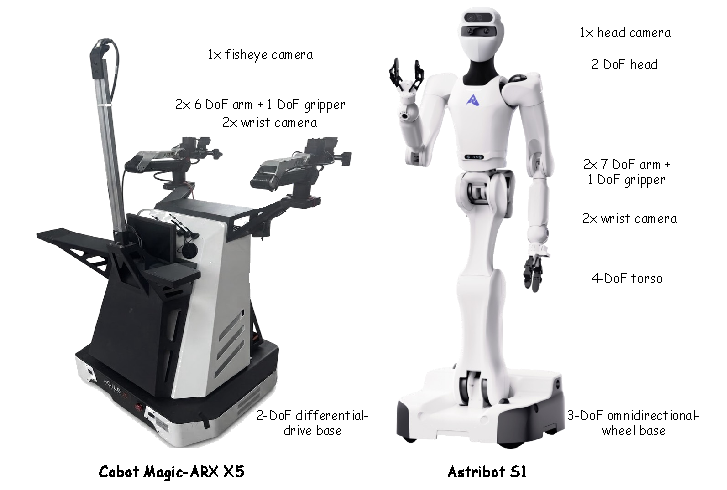
\includegraphics[width=\linewidth]{figures/mobile_BM_embodiment.pdf}
\captionof{figure}{Illustration of the long-horizon mobile manipulation experiments platform.}
\label{fig:bm_mobile_tasks}
\end{minipage}

\end{figure}














\section{Ablation Studies}

\subsection{Action Space}
\begin{figure*}[h]
    \centering
    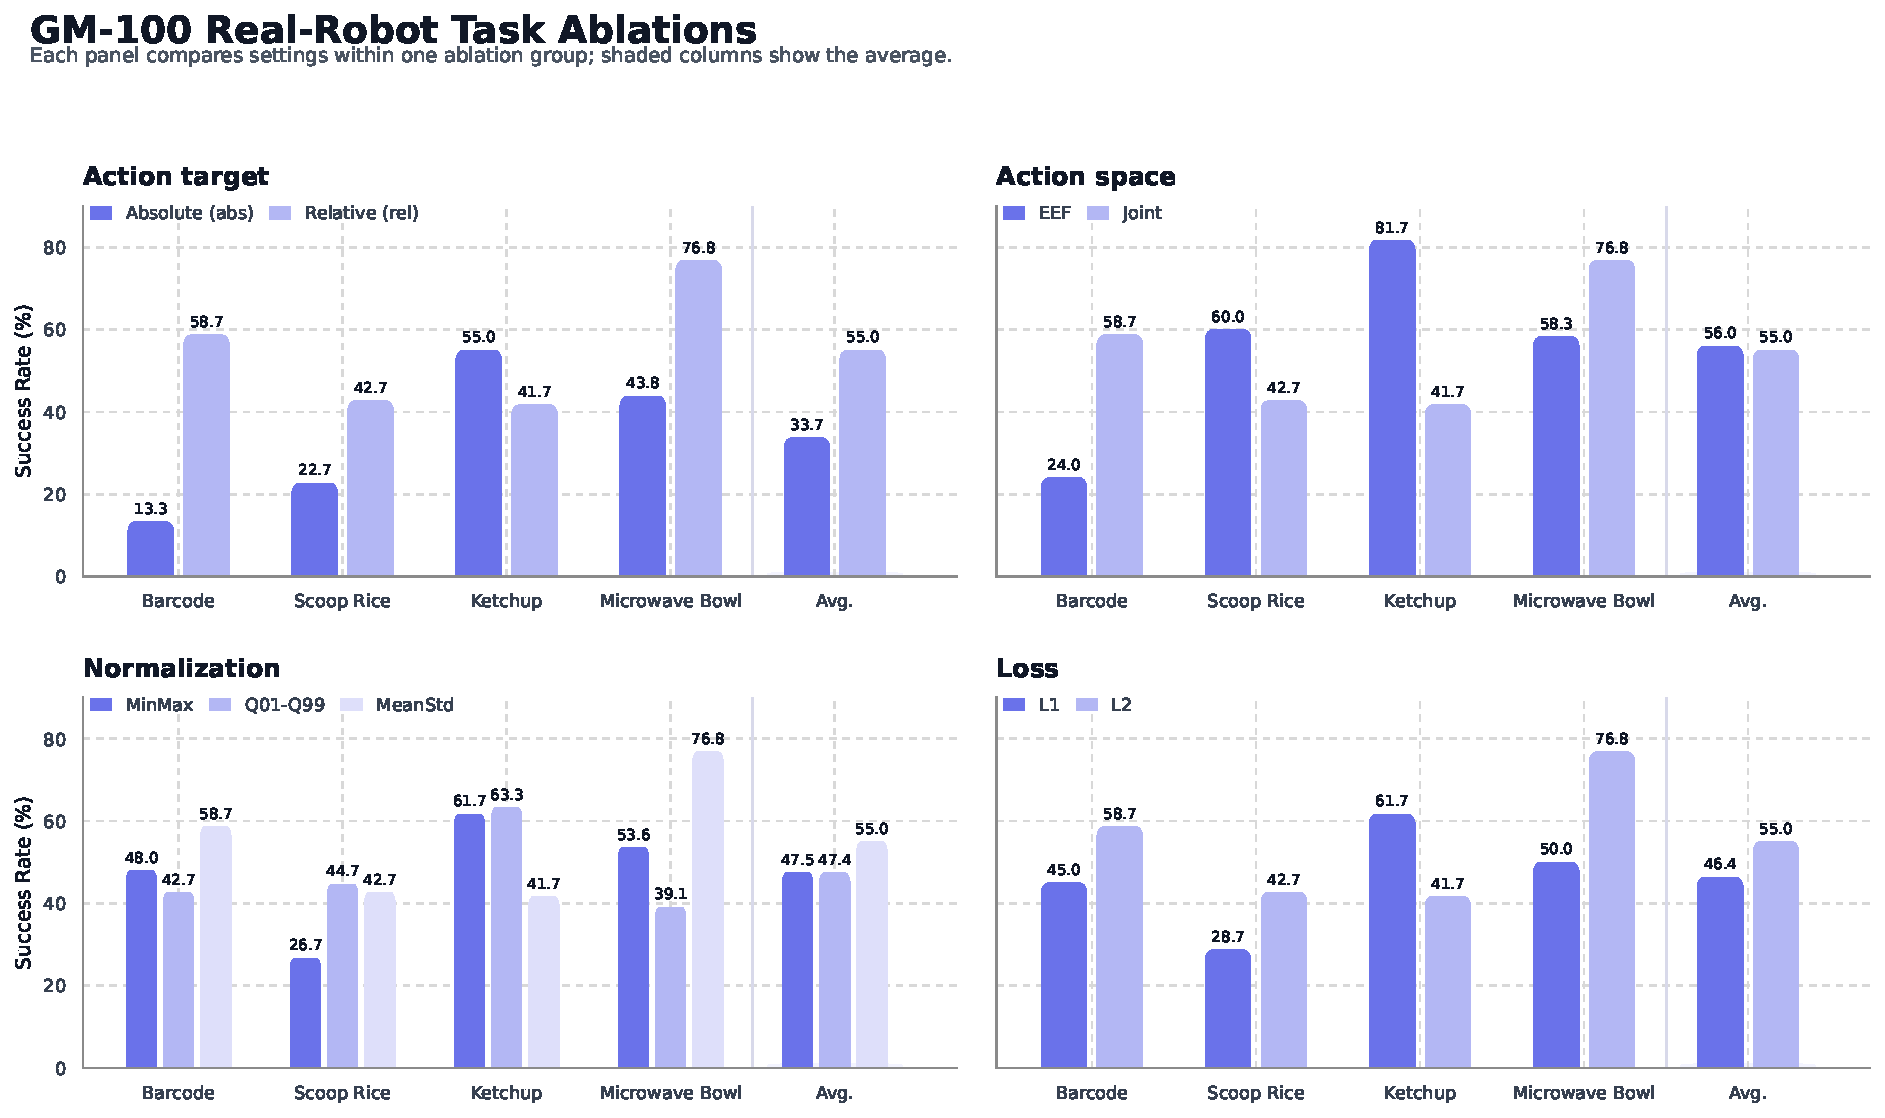
\includegraphics[width=\textwidth, trim=0 0 0 50pt, clip]{figures/gm100_ablation_barplot.pdf}
    \caption{Results on the four GM-100 real-robot tasks.}
    \label{fig:gm100}
\end{figure*}

\noindent\textbf{Action target.}
For the action target, relative joint actions substantially outperform absolute joint actions, improving the average success rate from $33.7$ to $55.0$. This is supported by the action statistics in \cref{fig:action_target_norm_stats}A. Across the four tasks, the standard deviation of \texttt{relQpos} is only $31\%$--$37\%$ of that of \texttt{absQpos}; on the pooled distribution, the action standard deviation decreases from about $0.80$ for \texttt{absQpos} to $0.28$ for \texttt{relQpos}. Therefore, relative actions convert the prediction target from global joint-configuration regression into local motion regression, producing targets that are more centered and have lower variance.

\begin{figure*}[h!]
    \centering
    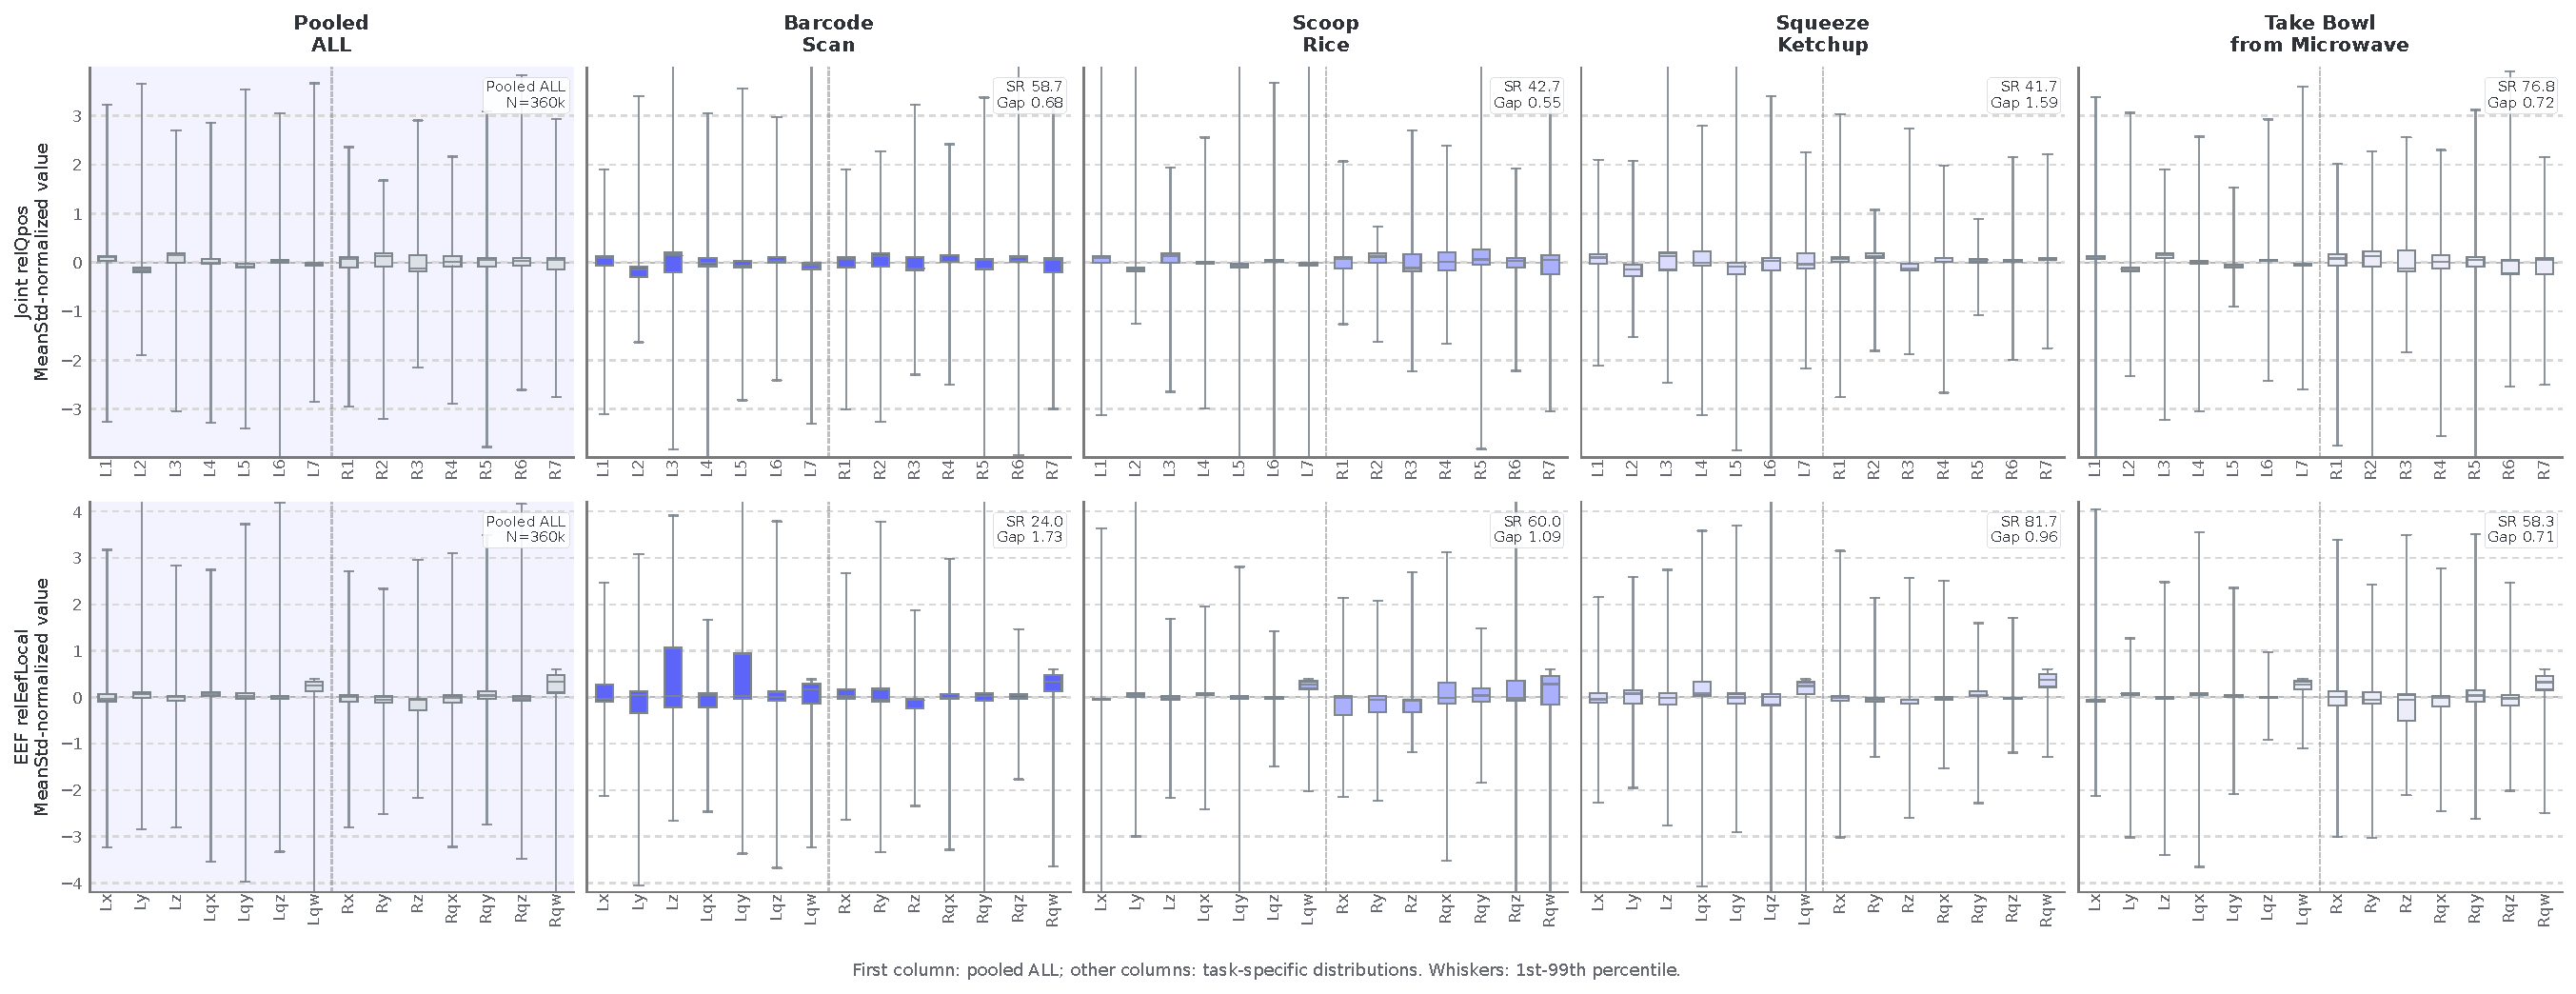
\includegraphics[width=\textwidth]{figures/fig_action_space_boxalign.pdf}
    \caption{Per-dimension MeanStd-normalized action distributions for joint and EEF action spaces. The first column shows the pooled distribution over all four tasks, while the remaining columns show task-specific distributions. The gap measures task-to-pooled distribution alignment based on per-dimension median and IQR differences.}
    \label{fig:action_space_boxalign}
\end{figure*}

\noindent\textbf{Action space.}
For the action space, EEF and joint actions obtain similar average success rates, $56.0$ and $55.0$, respectively, but show different task-level preferences. To analyze this, \Cref{fig:action_space_boxalign} compares the per-dimension MeanStd-normalized action distributions of each task against the pooled distribution over all four tasks. We additionally report a distribution-alignment gap, computed from the per-dimension median and IQR differences between each task and the pooled distribution; a smaller gap indicates that the task-specific action distribution is closer to the overall distribution.

The results show that distribution alignment explains part, but not all, of the action-space behavior. For Barcode Scan, joint actions are much closer to the pooled distribution than EEF actions, with a gap of $0.68$ versus $1.73$, consistent with the large performance advantage of joint actions ($58.7$ vs. $24.0$). For Squeeze Ketchup, the opposite trend appears: EEF actions have a smaller gap than joint actions ($0.96$ vs. $1.59$) and achieve much higher success ($81.7$ vs. $41.7$), suggesting that contact-rich endpoint motions are better represented in Cartesian EEF space. For Scoop Rice, however, EEF actions outperform joint actions despite a larger distribution gap, indicating that Cartesian motion regularity can outweigh pure distribution alignment. For Take Bowl from Microwave, the two gaps are nearly identical ($0.71$--$0.72$), while joint actions still perform better, suggesting that posture, reachability, and configuration-dependent constraints are more important than marginal action statistics. Overall, the best action space depends on both distributional alignment and the physical structure of the task.

\begin{figure*}[h!]
    \centering
    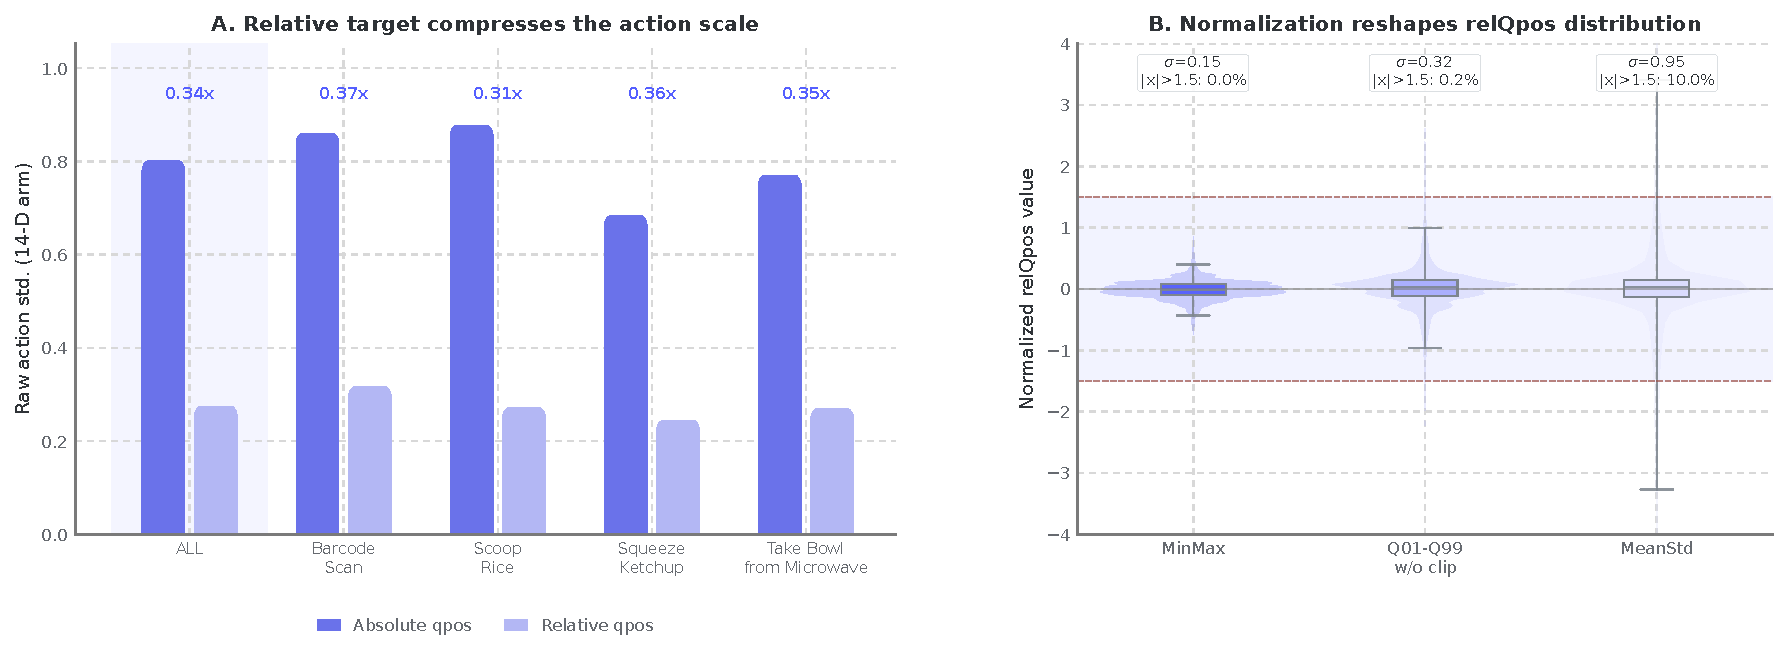
\includegraphics[width=\textwidth]{figures/fig_ac_seaborn_allstyle.pdf}
    \caption{Action targets and normalization statistics for the four GM-100 tasks. Left: \texttt{relQpos} substantially reduces the action scale compared with \texttt{absQpos}. Right: normalization changes the effective dynamic range of MeanStd-normalized \texttt{relQpos}; Q01--Q99 is shown in the actual unclipped setting.}
    \label{fig:action_target_norm_stats}
\end{figure*}
\noindent\textbf{Normalization.}
For normalization, \Cref{fig:action_target_norm_stats}B shows the normalized \texttt{relQpos} distributions under the three schemes. MinMax compresses most samples into a narrow range: its normalized standard deviation is only $0.15$, and the 1st--99th percentile interval is approximately $[-0.42, 0.40]$. This strong compression reduces the effective resolution of the action targets, which explains its lower average success rate of $47.5$.

Q01--Q99 increases the normalized standard deviation to $0.32$ and expands the central mass to roughly $[-0.96, 1.01]$. Importantly, the actual implementation used here is not clipped; only about $0.2\%$ of values fall outside $[-1.5, 1.5]$. Thus, its weakness is not information loss from clipping, but rather that the normalized targets remain much more compressed than under MeanStd. This explains why Q01--Q99 improves the central dynamic range over MinMax but still achieves a similar average success rate of $47.4$.

MeanStd provides the largest effective dynamic range, with normalized standard deviation $0.95$ and a 1st--99th percentile interval of approximately $[-3.22, 3.30]$. Around $10.0\%$ of samples lie outside $|x|>1.5$, reflecting the long-tailed structure of the relative action distribution rather than clipping. By preserving these larger corrective motions, MeanStd achieves the best average success rate of $55.0$.

\noindent\textbf{Loss function.}
For the loss function, L2 achieves the best average performance, improving over L1 from $46.4$ to $55.0$. Since most \texttt{relQpos} targets are small continuous corrections around zero, L2 better fits the high-density region of the action distribution and encourages precise regression. L1 performs better on Squeeze Ketchup, consistent with its robustness to contact-rich or heavy-tailed motions, but underperforms on the other three tasks.












\subsection{Perceptual Results of Dual-query Distillation}
We adopt LingBot-Depth and DINO-Video as the visual teacher models for distillation training. Despite perceptual results not being essential for action generation, integrating specific task queries allows the VLA to obtain visual perceptual outcomes during causal inference. As shown in~\cref{fig:vis_distillation}, we present the causal perception results of \method, which validate the effectiveness of our model in distilling semantic priors and geometric cues.


\begin{figure}[t]
\centering
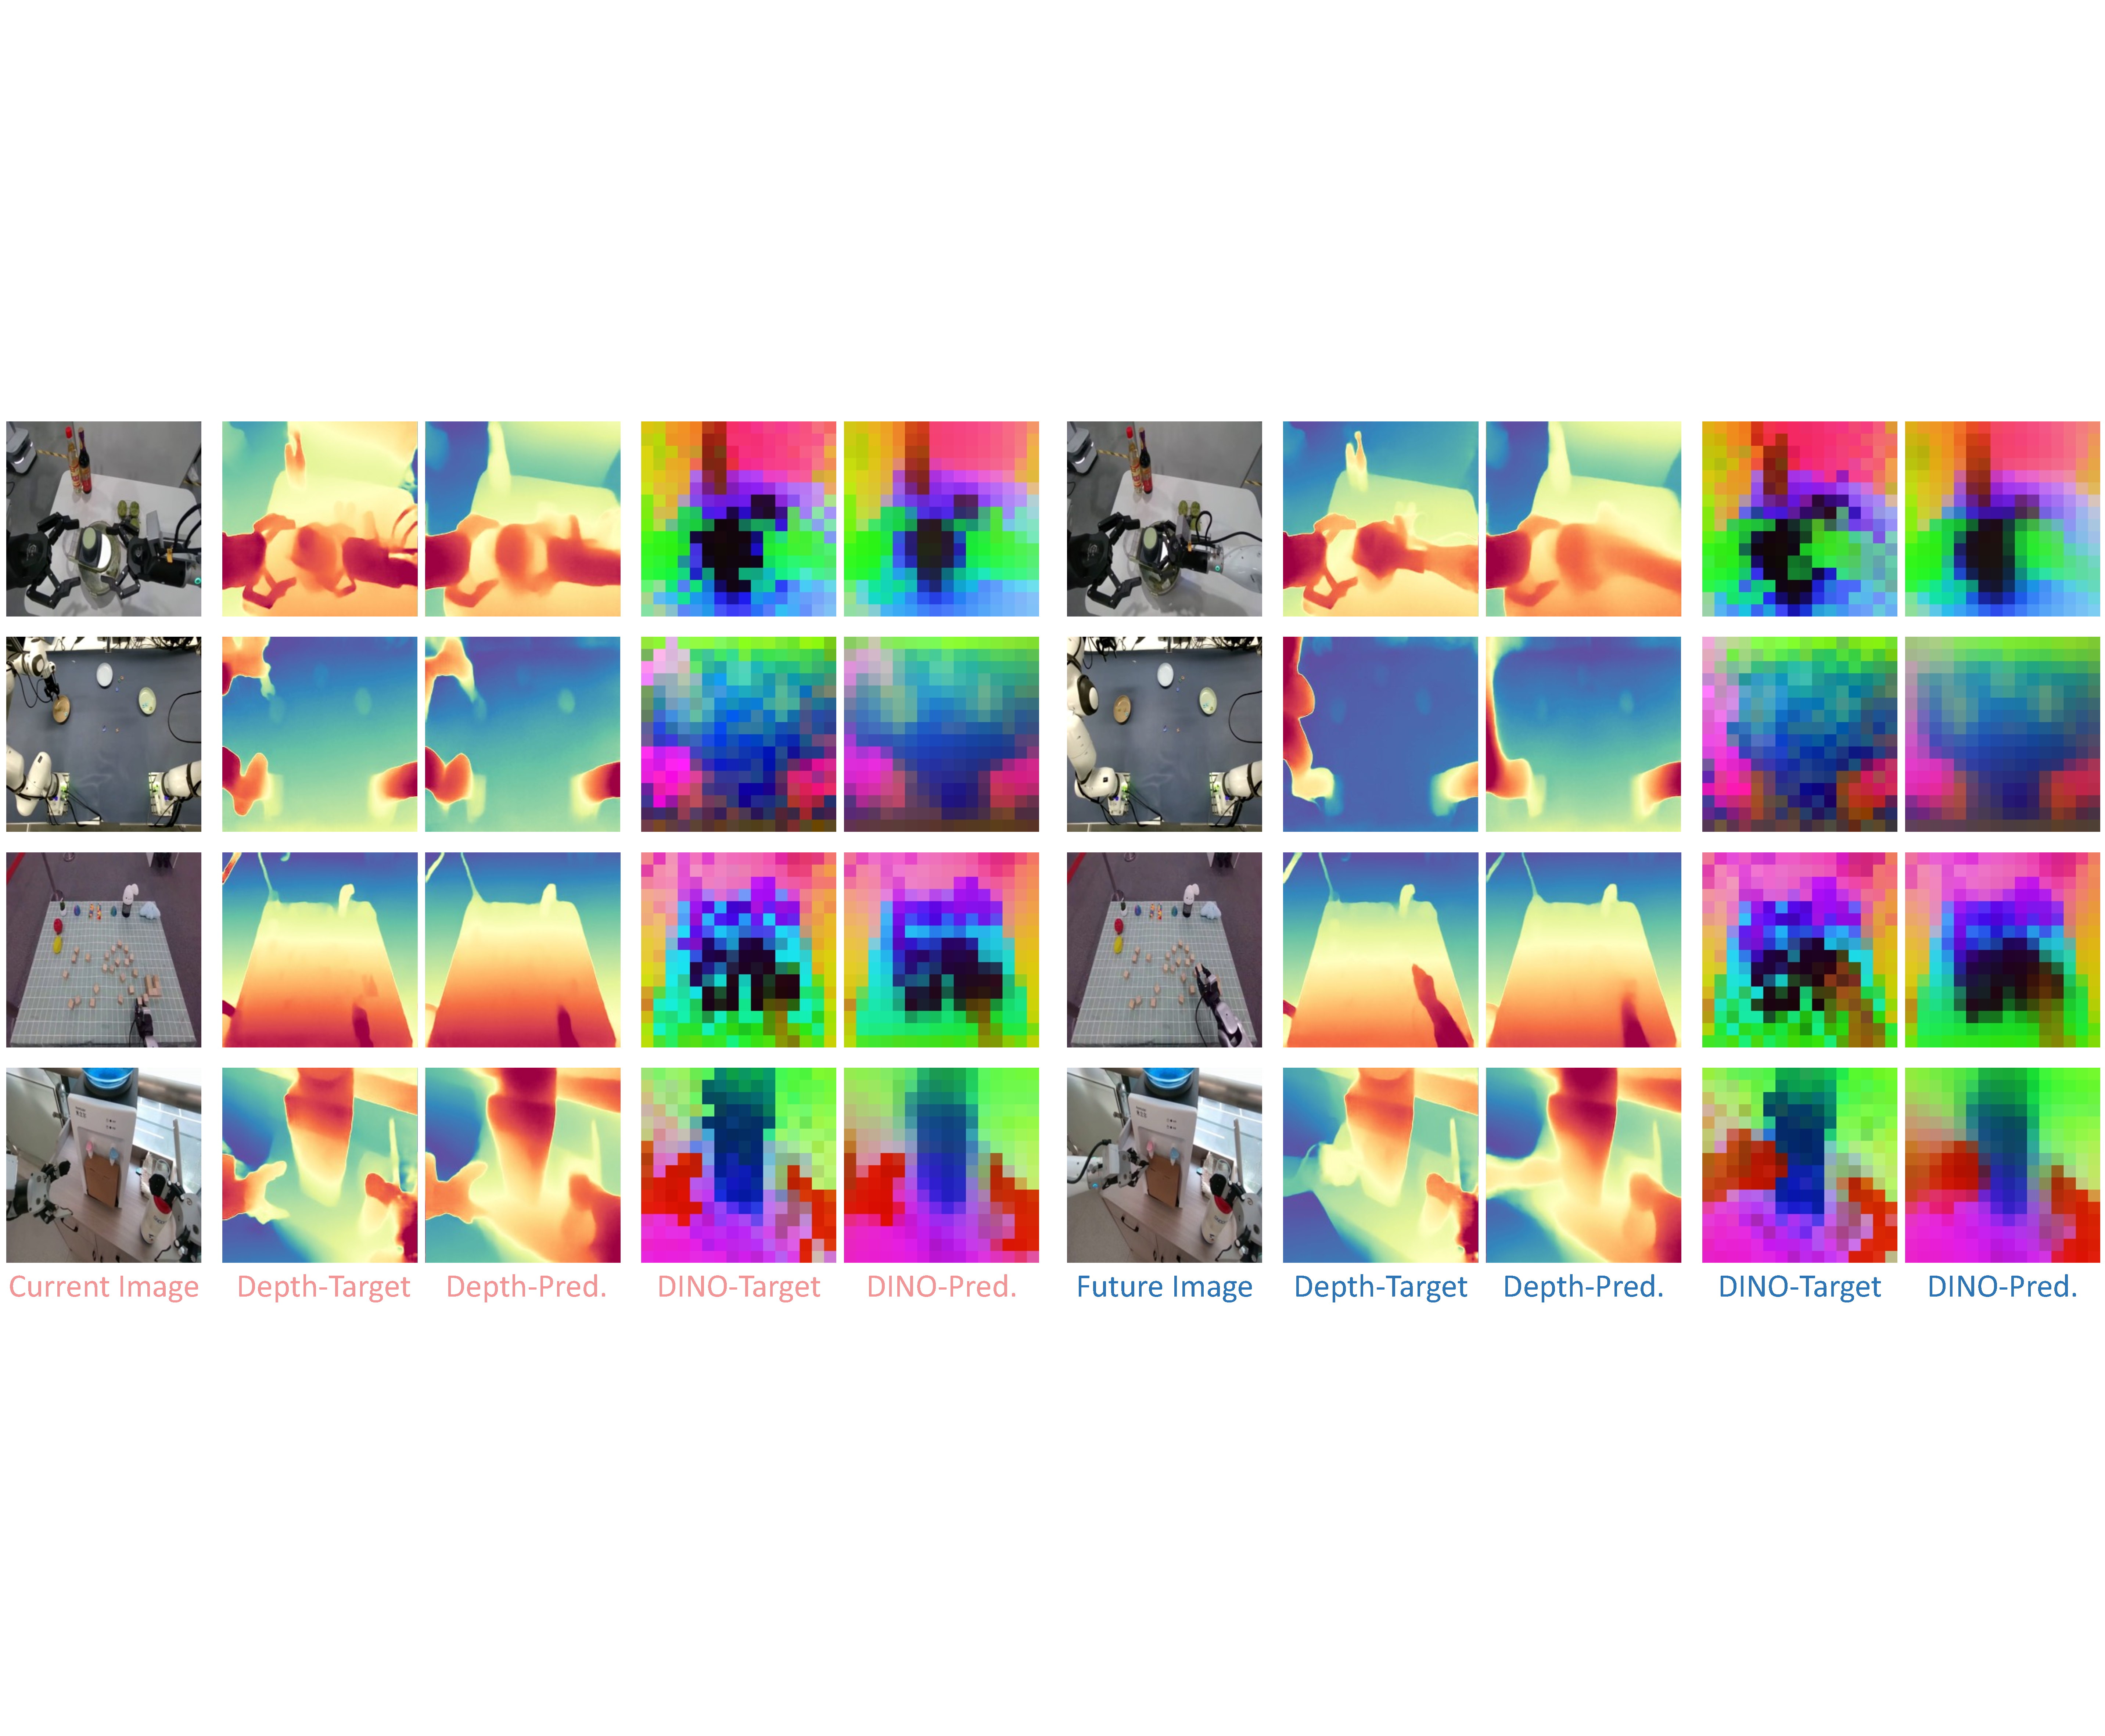
\includegraphics[width=\linewidth]{figures/vis_distillation.pdf}
\caption{Causal perception results of \method under visual distillation. \textbf{Left}:  depth/DINO-Video-PCA ground truth and prediction for current image. \textbf{Right}: depth/DINO-Video-PCA ground truth and prediction for future image.}
\label{fig:vis_distillation}
\end{figure}
